\documentclass{article}
\usepackage{etoolbox}
\usepackage{graphicx}
\usepackage{amsmath}

\ifdef{\myoutput}{}{\def\myoutput{concept}}
\ifdef{\myversion}{}{\def\myversion{1}}

\usepackage[output=\myoutput
,numberofversions=4
,version=\myversion
,seed=4
,randomizequestions=true
,randomizeanswers=true
,writeRfile=true
]{mcexam}

\usepackage[margin=0.95in]{geometry}
\usepackage{multicol}

\usepackage{fancyhdr,lastpage}
\pagestyle{fancy}
\fancyhf{}
\renewcommand{\headrulewidth}{1pt} 
\renewcommand{\footrulewidth}{1pt}
\lfoot{\mctheversion}
\rfoot{Page \thepage\ of \pageref{LastPage}}
\lhead{Final Exam \mctheversion \\ MAT 2000: Introduction to Statistics}
\rhead{Name Print): \hspace{2.5 in}}

\usepackage{calc}
\renewenvironment{setmcquestion}
{\begin{minipage}[t]{\linewidth-\labelwidth}}
	{\end{minipage}\par}

\renewenvironment{setmcquestioninstruction}
{\begin{minipage}{\textwidth}}
	{\end{minipage}}

\renewenvironment{setmcanswers}{}{}
\setlist[setmcquestions]{label=\mcquestionlabelfmt{*}.
	,ref=\mcquestionlabelfmt{*}
	,itemsep=0.5\baselineskip
	,topsep=1\baselineskip
}

\renewcommand\mcversionlabelfmt[1]{\arabic{#1}}

%copy-pasting from MS Word, use regex to find [\*]*[a-d]\. and replace with \answer 

\raggedbottom

\begin{document}
	Circle the correct answer for each question.  If you're unsure, you can write numbers 1, 2, 3, etc. next to the choices to get partial credit.  Questions refer to the nonindented paragraph above unless otherwise stated.  All questions are 2 points unless otherwise stated.\\[.5cm]
	
	\begin{mcquestions}
		
		\question (6 points) A survey on 1,500 high school seniors who took the SAT and who completed an optional web survey shows that 58\% of high school seniors are fairly certain that they will participate in a study abroad program in college. Does this survey provide convincing evidence that the majority (more than 50\%) of all high school seniors who take the SAT are fairly certain they will participate in a study abroad program in college?  Use this scenario to (a) state the null and alternative hypotheses in proper notation and (b) state the value of the statistic using proper notation.
		\begin{mcanswerslist}[permutenone]
			\answer : \vspace{.5 in}
			\answer : 
		\end{mcanswerslist}
		\begin{mcexplanation}
			The correct answers are
			\begin{enumerate}[label=(\alph*)]
				\item \(H_0: \pi = 0.50\) versus \(H_A: \pi > 0.50\)
				\item \(\hat p=0.58\)
			\end{enumerate}
		\end{mcexplanation}
		
		\question[follow] The p-value for the question above is less than 0.001. Interpret this value in context of the problem. \label{sa3}
		\begin{mcanswerslist}
			\answer There is less than a 0.1\% chance that 50\% of all high school seniors who take the SAT are fairly certain they will participate in a study abroad program in college.
			\answer[correct] In less than 0.1\% of all samples of 1,500 high school seniors who take the SAT, 58\% or more would respond that they are fairly certain they will participate in a study abroad program in college, if the true probability is 0.50.
			\answer In less than 0.1\% of all samples of 1,500 high school seniors who take the SAT, 50\% or more would respond that they are fairly certain they will participate in a study abroad program in college, if the true probability is 0.58.
			\answer There is less than a 0.1\% chance that more than 50\% of all high school seniors who take the SAT are fairly certain they will participate in a study abroad program in college.
		\end{mcanswerslist}
		
		\begin{mcquestioninstruction}
			An environmental science teacher at a high school with a large population of students was curious whether the majority (more than half) of students at the school regularly recycle plastic bottles. The teacher selected a random sample of 146 students at the school to interview, then asked each student: "Do you recycle plastic bottles more often than you throw them in the trash?" (Yes/No). Suppose that 89 of the students answered "Yes".
			
			Use this scenario to answer questions \ref{r1} and \ref{r2}
		\end{mcquestioninstruction}
		
		\question  How would the strength of evidence against the null hypothesis change if the teacher wanted to know whether the proportion of students at the school that would have said "Yes" differed from 0.5 rather than was greater than 0.5.\label{r1}
		
		\begin{mcanswerslist}
			\answer Stronger evidence against the null hypothesis
			\answer[correct] Weaker evidence against the null hypothesis
			\answer The same amount of evidence against the null hypothesis
			\answer Cannot be determined from the information given
		\end{mcanswerslist}
		
		\question[follow]  If all other aspects of the study remained the same, how would the strength of evidence against the null hypothesis change if the teacher sampled 300 students instead of 146.\label{r2}
		\begin{mcanswerslist}
			\answer[correct] Stronger evidence against the null hypothesis
			\answer Weaker evidence against the null hypothesis
			\answer The same amount of evidence against the null hypothesis
			\answer Cannot be determined from the information given
		\end{mcanswerslist}
		
		\begin{mcquestioninstruction}
			A study conducted by the National Center for Health Statistics as part of the Center for Disease Control and Prevention (CDC) found that, as of 2015-2016, 39.6\% of Americans over the age of 20 fit the medical definition of being obese (BMI of 30 or higher). A city known for plentiful outdoor opportunities believes that number is lower among residents. A representative sample of 80 city residents is collected and the BMI calculated for each (based on reported height and weight). The variable of interest is whether the resident fit the medical definition of obese. The study found 22 people in the sample fit the medical definition of obese.
			
			Use this scenario for the questions \ref{BMI1} and \ref{BMI2}:
		\end{mcquestioninstruction}
		
		\question[follow] Select the appropriate method of calculating the standard deviation of the sample proportions under the null hypothesis. \label{BMI1}
		
		\begin{mcanswerslist}
			\answer[correct] \(\sqrt{\frac{0.396 \times (1-0.396)}{80}}\)\\[0.1cm]
			\answer \(\sqrt{\frac{0.275 \times (1-0.275)}{80}}\)\\[0.1cm]
			\answer \(\sqrt{\frac{22 \times (1-22)}{80}}\)\\[0.1cm]
			\answer \(\sqrt{\frac{80 \times (1-80)}{0.396}}\)\\[0.1cm]
		\end{mcanswerslist}
		
		\question[follow] Letting \(SE\) be the standard error (your answer to question \ref{BMI1}), which of the following displays the correct method of calculating the standardized statistic? \label{BMI2}
		
		\begin{mcanswerslist}
			\answer \(\frac{22-31.7}{80\times SE}\)\\[0.1cm]
			\answer \(\frac{0.5-0.275}{SE}\)\\[0.1cm]
			\answer[correct] \(\frac{0.275-0.396}{SE}\)\\[0.1cm]
			\answer \(\frac{SE-0.396}{0.5}\)\\[0.1cm]
		\end{mcanswerslist}
		
		\question If the p-value is very small, which of the following is true?
		\begin{mcanswerslist}
			\answer[correct] Very strong evidence exists against the null hypothesis.
			\answer Very strong evidence exists against the alternative hypothesis.
			\answer The null hypothesis has been proven.
			\answer The alternative hypothesis has been proven.
		\end{mcanswerslist}
		
		\question The following 19 test scores are based on a random sample of final exam scores (sorted in increasing order) for the population of students who took an elementary statistics course at a large university over a 5 year period:
		
		\begin{tabular}{ccccccccccccccccccc}
			61 &  65 &  69  & 70  & 71 &  73  & 75 &  77 &  77 &  82  & 82 &  83 &  84 &  85 &  86 &  89 &  92  & 92 &  94
		\end{tabular}
		
		Suppose the largest test score in the sample changed from a 94 to a 90. Describe how each of the following statistics would change.\\
		The median would \_\_\_(1)\_\_\_.\\
		The mean would \_\_\_(2)\_\_\_.\\
		The standard deviation would \_\_\_(3)\_\_\_.
		
		\begin{mcanswerslist}
			\answer decrease, decrease, decrease
			\answer remain the same, decrease, increase
			\answer[correct] remain the same, decrease, decrease
			\answer decrease, increase, remain the same			
		\end{mcanswerslist}
		
		\question Suppose a population of test scores is skewed left. What would be the shape of the sampling distribution for sample mean test scores from samples of 50 students?
		\begin{mcanswerslist}
			\answer Skewed right
			\answer Skewed left
			\answer[correct] Approximately normal
			\answer Unable to determine
		\end{mcanswerslist}
		
		\question Suppose a confidence interval is constructed using repeated tests of significance to develop an interval of plausible values.  Two-sided tests are used each time with the following null hypotheses and resulting p-values.
		\begin{center}
			\begin{tabular}{llp{.75in}ll}
				Null              & p-value & & Null              & p-value  \\
				$\pi = 0.45$ & 0.009   &                                 & $\pi = 0.53$ & 0.787    \\
				$\pi = 0.46$ & 0.032   &                                 & $\pi = 0.54$ & 0.572    \\
				$\pi = 0.47$ & 0.062   &                                 & $\pi = 0.55$ & 0.373    \\
				$\pi = 0.48$ & 0.126   &                                 & $\pi = 0.56$ & 0.142    \\
				$\pi = 0.49$ & 0.371   &                                 & $\pi = 0.57$ & 0.077    \\
				$\pi = 0.50$ & 0.598   &                                 & $\pi = 0.58$ & 0.042    \\
				$\pi = 0.51$ & 0.733   &                                 & $\pi = 0.59$ & 0.021    \\
				$\pi = 0.52$ & 0.986   &                                 & $\pi = 0.60$ & 0.003   
			\end{tabular}
		\end{center}
		Using the results, give a 95\% confidence interval.
		\begin{mcanswerslist}
			\answer (0.50, 0.54)
			\answer[correct] (0.47, 0.57)
			\answer (0.45, 0.60)
			\answer (0.46, 0.58)
		\end{mcanswerslist}
		
		\question Suppose a test of significance is conducted with $H_0: \pi = 0.50$ and $H_A: \pi \neq 0.50$ with a resulting p-value of 0.07.  Also, 99\% and 95\% confidence intervals are constructed from the data.
		What will be true about the confidence intervals?
		\begin{mcanswerslist}
			\answer[correct] Both the 99\% and the 95\% intervals will contain 0.50.
			\answer Neither the 99\% nor the 95\% intervals will contain 0.50.
			\answer The 99\% interval will contain 0.50, but the 95\% interval will not contain 0.50.
			\answer The 99\% interval will not contain 0.50, but the 95\% interval will contain 0.50.
		\end{mcanswerslist}
		
			\question The spinning dancer (or silhouette illusion) is a moving image of a woman that appears to be spinning.  Some people see her spinning clockwise and some see her spinning counterclockwise.  A student showed other students this and found that 30 out of 50 (or 60\%) saw her spinning clockwise.  The student researcher was interested in the probability of a randomly chosen student that would see the dancer spinning clockwise.  The student created the following null distribution.
		\includegraphics[width=\textwidth]{../images/null_dancer.jpg}
		Using the information provided above, determine a 2SD confidence interval for the long-run probability a randomly chosen student would see the woman spinning clockwise.  (Don't use any other applet to do this, just the information above.)
		\begin{mcanswerslist}
			\answer (0.36, 0.64)
			\answer[correct] (0.46, 0.74)
			\answer (0.53, 0.67)
			\answer (0.43, 0.57)
		\end{mcanswerslist}
		
		\question Many studies have investigated the question of whether people tend to think of an odd number when asked to think of a single-digit number (0 through 9; 0 is considered an even number). When asked to pick a number between 0 and 9, out of 70 students, 42 chose an odd number. Let the parameter of interest, $\pi$ , represent the probability that a student will choose an odd number.\\
		Are conditions met to use theory-based methods for conducting a 95\% confidence interval?
		\begin{mcanswerslist}
			\answer Yes, because there were two possible outcomes.
			\answer Yes, since the number of students is larger than 30.
			\answer[correct] Yes, since the number of students who chose an odd number, and the number of students who chose an even number, are both greater than 10.
			\answer No, since the sample size is too small.
		\end{mcanswerslist}
		
		\question Suppose a 95\% confidence interval for a population proportion is (0.21, 0.43). How would the width of the confidence interval change if the confidence level was changed?
		\begin{mcanswerslist}
			\answer Both a 99\% confidence interval and a 90\% confidence interval would both be wider.
			\answer[correct] A 99\% confidence interval would be wider and a 90\% confidence interval would be narrower.
			\answer A 99\% confidence interval would be narrower and a 90\% confidence interval would be wider.
			\answer Both a 99\% confidence interval and a 90\% confidence interval would be narrower.
		\end{mcanswerslist}
		
		\question Suppose data is collected on the heights of all students at a college.  Each of the 250 people taking a statistics course randomly takes a sample of 40 of these heights and constructs a 95\% confidence interval for mean height of all students at the college.
		
		Which of the following statements about the confidence intervals is most accurate?
		\begin{mcanswerslist}
			\answer About 95\% of the heights of all students at the college will be contained in these intervals.
			\answer About 95\% of the time, a student's sample mean height will be contained in the interval the student found.
			\answer[correct] About 95\% of the intervals will contain the population mean height.
			\answer About 95\% of the intervals will be identical.
		\end{mcanswerslist}
		
		\question (8 points) A study published in 2007 by Christopher Johnson, professor of music education and music therapy at the University of Kansas, revealed that students in elementary schools who took private music lessons scored around 20 percent higher in math scores on standardized tests, compared to students who did not take private music lessons.  What is (a) the explanatory variable, (b) the response variable, (c) a randomized experiment or an observational study? And (d) give a reason for your answer to (c).
		\begin{mcanswerslist}[permutenone]
			\answer \rule{\textwidth}{0.5 pt}
			\answer \rule{\textwidth}{0.5 pt}
			\answer \rule{\textwidth}{0.5 pt}
			\answer \rule{\textwidth}{0.5 pt}
			\rule{\textwidth}{0.5 pt}
		\end{mcanswerslist}
		\begin{mcexplanation}
			The correct answers are
			\begin{enumerate}[label=(\alph*)]
				\item Whether a student took private music lessons
				\item Math score on standardized test
				\item Observational study
				\item Since whether the student took private music lessons was not randomly assigned.
			\end{enumerate}
		\end{mcexplanation}
		
		\question Which of the following data sets has the largest standard deviation?
		\begin{mcanswerslist}
			\answer 1, 2, 3, 4, 5
			\answer 1, 3, 3, 3, 5
			\answer[correct] 1, 1, 3, 5, 5
			\answer 1, 1, 1, 1, 1
		\end{mcanswerslist}
		
		\begin{mcquestioninstruction}
			A random sample of Grace College students was taken and one of the questions asked was how many hours per week they study.  The goal is to see whether a difference exists between males and females in terms of average study time.  The sample results are given in the following table.
			\begin{center}
				\begin{tabular}{| l | l | l |}
					\hline
					& \textbf{Female} & \textbf{Male} \\
					\hline
					\textbf{Sample Size} & 125 & 75 \\
					\hline
					\textbf{Sample Average} & 18.52 & 15.17 \\
					\hline
					\textbf{Sample SD} & 10.85 & 11.32 \\
					\hline
				\end{tabular}
			\end{center}
		\end{mcquestioninstruction}
		
		\question Assuming the distribution of study times is not strongly skewed for either sample, which approach would be more appropriate for these data: simulation-based or theory-based?
		\begin{mcanswerslist}
			\answer Simulation-based, since this approach works for any sample size.
			\answer Theory-based, since both 125 and 75 are greater than 20.
			\answer[correct] Either approach would be appropriate.
			\answer Neither approach would be appropriate.
		\end{mcanswerslist}
		
		\begin{mcquestioninstruction}
			A 1997 study described in the European Journal of Clinical Nutrition compares the growth of a random sample of vegetarian and omnivorous children, ages 7 - 11, in Northwest England. One of the aspects on which the children were compared was their body mass index (BMI). Of the 50 vegetarian children in the study, the average BMI was 16.76 and the standard deviation was 1.91. Among the 30 omnivorous children in the study, the average BMI was 17.12 and the standard deviation was 2.23.  Use this scenario to answer questions \ref{veg1}, \ref{veg2}, and \ref{veg3}
		\end{mcquestioninstruction}
		
		\question Which best describes this study design? \label{veg1}
		\begin{mcanswerslist}
			\answer Paired using repeated measures
			\answer Paired using matching
			\answer[correct] Independent groups
			\answer None of the above
		\end{mcanswerslist}
		
		\question[follow] (4 points) Write down (a) the correct formula and (b) compute the standard error (the standard deviation of the null distribution) for this sample. \label{veg2}
		\begin{mcanswerslist}[permutenone]
			\answer : \vspace{.25 in}
			\answer :
		\end{mcanswerslist}
		\begin{mcexplanation}
			The correct answers are
			\begin{enumerate}[label=(\alph*)]
				\item \(SE = \sqrt{\frac{s_1^2}{n_1} + \frac{s_2^2}{n_2}}\)
				\item \(SE \approx 0.4885952654\)
			\end{enumerate}
		\end{mcexplanation}
		
		\question[follow] (12 points) The p-value for this study is 0.2322.  (a) Interpret the p-value in the context of this study (i.e. ``The p-value is the probability...'') and (b) In light of this p-value, write a one-sentence conclusion for this study. \label{veg3}
		\begin{mcanswerslist}[permutenone]
			\answer \rule{\textwidth}{.5pt}
			\rule{\textwidth}{.5pt}
			\rule{\textwidth}{.5pt}
			\vspace{.1 in}
			\answer \rule{\textwidth}{.5pt}
			\rule{\textwidth}{.5pt}
			\rule{\textwidth}{.5pt}
		\end{mcanswerslist}
		\begin{mcexplanation}
		The correct answers are
		\begin{enumerate}[label=(\alph*)]
			\item The p-value is the probability that we would observe this much difference between the average BMI of 50 vegetarian children and 30 omnivorous children assuming that there is no inherent difference.
			\item There is not sufficient evidence to conclude that there is a difference in BMI between vegetarian children and omnivorous children.
		\end{enumerate}
		\end{mcexplanation}
		
		\question A random sample of medical records from 28 heart attack patients at a Boston hospital was used to better understand the relationship between cholesterol and heart failure.  The cholesterol levels of heart attack patients were recorded at 2 days and at 14 days after the patient had a heart attack.
		
		Which best describes this study design?
		\begin{mcanswerslist}
			\answer[correct] Paired using repeated measures
			\answer Paired using matching
			\answer Independent groups
			\answer None of the above
		\end{mcanswerslist}
		
		\question Researchers randomly selected 36 children who had been identified as gifted from a large city. The IQ of each child and the IQ of the child's mother were measured. A statistical analysis will be performed to determine if IQs of gifted children tend to be higher than their mothers' IQ on average.
		
		Which best describes this study design?
		
		\begin{mcanswerslist}
			\answer Paired using repeated measures
			\answer[correct] Paired using matching
			\answer Independent groups
			\answer None of the above
		\end{mcanswerslist}
		
		\question Suppose the chi-square statistic for a test was 6.991. If instead, the chi-square statistic had been 5.332, would the p-value be smaller, larger, or remain the same?
		\begin{mcanswerslist}
			\answer Smaller
			\answer[correct] Larger
			\answer Remain the same
			\answer Cannot be determined
		\end{mcanswerslist}
		
		\begin{mcquestioninstruction}
			Some student researchers want to determine if students yawning (when being yawned at) is associated with the time of day (morning, afternoon, and evening). The students found the following results from yawning in front of people around campus:
			\begin{itemize}
				\item Morning: 25 of the 39 people yawned back
				\item Afternoon: 15 of the 38 people yawned back
				\item Evening: 29 of the 44 people yawned back
			\end{itemize}
		\end{mcquestioninstruction}
		
		\question When an ANOVA test is run, a p-value of 0.03 is found. What would be an appropriate conclusion?
		\begin{mcanswerslist}
			\answer Strong evidence exists that the probability a person yawns is different between all three times of day: morning, afternoon, and evening.
			\answer[correct] Strong evidence exists of an association between time of day and whether a person yawns.
			\answer Strong evidence of no association between time of day and whether a person yawns.
			\answer Strong evidence does not exist of an association between time of day and whether a person yawns.
		\end{mcanswerslist}
		
		\begin{mcquestioninstruction}
			Are people equally likely to be born on any day of the seven days of the week? Or are some days more likely to be a person's birthday than other days?  To investigate this question, days of birth were recorded for the 147 "noted writers of the present" listed in The World Almanac and Book of Facts 2000. The counts for the seven days of the week are given in the following table.
			\begin{center}
				\begin{tabular}{ccccccc}
					Mon&Tues&Wed&Thurs&Fri&Sat&Sun\\ \hline
					17&26&22&23&18&15&25					
				\end{tabular}
			\end{center}
			Use this information to answer questions \ref{birthday-1} and \ref{birthday-2}
		\end{mcquestioninstruction}
		\question Are validity conditions met to conduct a theory-based chi-square goodness-of-fit test? \label{birthday-1}
		\begin{mcanswerslist}
			\answer[correct]  Yes, since all observed counts are at least 10.
			\answer  Yes, since we have at least 10 successes and 10 failures.
			\answer  No, since the p-values in questions 35 and 37 were different.
			\answer  No, since this was not a random sample.
		\end{mcanswerslist}
		
		\question[follow] Based upon a p-value of 0.53, what is the appropriate conclusion for the test? \label{birthday-2}
		\begin{mcanswerslist}
			\answer  Strong evidence exists that people are equally likely to be born on any day of the seven days of the week.
			\answer  Strong evidence does not exist that people are equally likely to be born on any day of the seven days of the week.
			\answer  Strong evidence exists that people are not equally likely to be born on any day of the seven days of the week.
			\answer[correct]  Strong evidence does not exist that people are not equally likely to be born on any day of the seven days of the week.
		\end{mcanswerslist}
		
		\question The two graphs, A and B, show dotplots from two different data sets. Suppose I want to compare the means in A and do another comparison of means in B. For each case an F-statistic is computed. Which of the following will be true about these statistics?
		\begin{center}
			\includegraphics[width = 0.75\textwidth]{../images/q-10-2-1.png}
		\end{center}
		\begin{mcanswerslist}
			\answer The F-statistic is the same in A and B.
			\answer The F-statistic is larger in A than in B.
			\answer[correct] The F-statistic is smaller in A than in B.
			\answer We cannot tell if the F-statistic will be larger in A or B.
		\end{mcanswerslist}
		
		\question When performing an ANOVA F-test, which definition of a p-value is the most accurate?
		\begin{mcanswerslist}
			\answer The p-value is the probability that the observed F-statistic will occur again.
			\answer[correct] If the null hypothesis is true, the p-value is the probability of observing an F-statistic as large or larger than the one actually observed.
			\answer The p-value is the value that an F-statistic must reach in order to be significant under the null hypothesis.
			\answer The p-value is the probability that the null hypothesis is true.
		\end{mcanswerslist}
		
		\begin{mcquestioninstruction}
			Babies born with low birth weights (less than 2500 grams) are at an increased risk for many infant diseases. Researchers in North Carolina collected data to see what variables may influence the birth weight (in grams) of a child, including whether the mother drank alcohol during pregnancy, whether the mother smoked during pregnancy, the mother's age (years), the gestation of the pregnancy (number of weeks from conception until birth), the mother's race, the length of the birth (hours), and several others. The plot below summarizes some of the variables measured.  Use this scenario to answer questions \ref{gest1} and \ref{gest2}.
			\begin{center}
				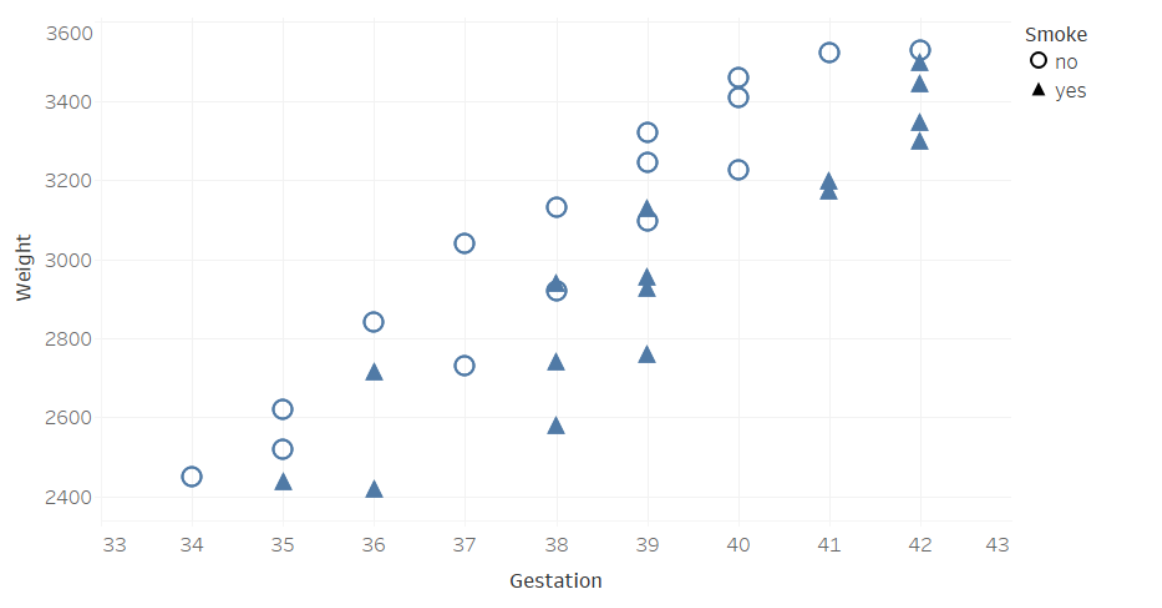
\includegraphics[width = 0.8\textwidth]{gestation.png}
			\end{center}
			
		\end{mcquestioninstruction}
		
		\question Based on the plot, does there appear to be an association between gestation period and birth weight? \label{gest1}
		\begin{mcanswerslist}
			\answer[correct] Yes, because as one variable increases, the other tends to increase as well.
			\answer No, because as one variable increases, the other tends to increase as well.
			\answer Yes, because most of the circles on the plot appear to be higher than the triangles.
			\answer No, because one variable does not appear to change the other variable.
		\end{mcanswerslist}
		
		\question[follow] How would the correlation coefficient between birth weight and gestation period computed from all women in the sample compare to the correlation coefficient between birth weight and gestation period computed from only non-smoking women? \label{gest2}
		\begin{mcanswerslist}
			\answer The correlation coefficient for the entire sample would be closer to 1 than the correlation coefficient for the non-smoking group.
			\answer[correct] The correlation coefficient for the entire sample would be closer to 0 than the correlation coefficient for the non-smoking group.
			\answer The correlation coefficient for the entire sample would be the same as the correlation coefficient for the non-smoking group.
			\answer We cannot determine how the two correlation coefficients compare based on this plot.
		\end{mcanswerslist}
		
		\begin{mcquestioninstruction}
			The following scatterplot displays the finish time (in minutes) and age (in years) for the male racers at the 2018 Strawberry Stampede (a 10k race through Arroyo Grande).
			\begin{center}
				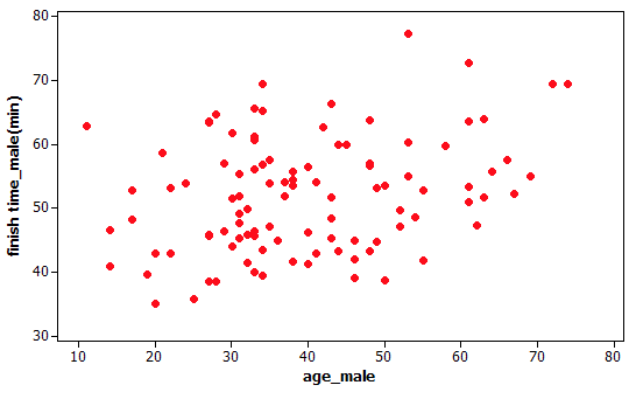
\includegraphics[width = 0.5\textwidth]{stampede.png}
			\end{center}
		\end{mcquestioninstruction}
		
		\question Approximate the value of the correlation coefficient for these data.
		\begin{mcanswerslist}
			\answer 0
			\answer[correct] 0.25
			\answer 0.6
			\answer 0.9
		\end{mcanswerslist}
		
		\question[follow] If a 70-year-old male with a finishing time of 35 minutes was added to the data set, would the correlation coefficient increase, decrease, or remain the same?
		\begin{mcanswerslist}
			\answer Increase
			\answer[correct] Decrease
			\answer Remain the same
			\answer Unable to determine with the information provided
		\end{mcanswerslist}
		
		\begin{mcquestioninstruction}
			The graph below shows a scatter plot of medical expenses in the past year by age for a sample of Americans.  Use this to answer question \ref{smile}
			\begin{center}
				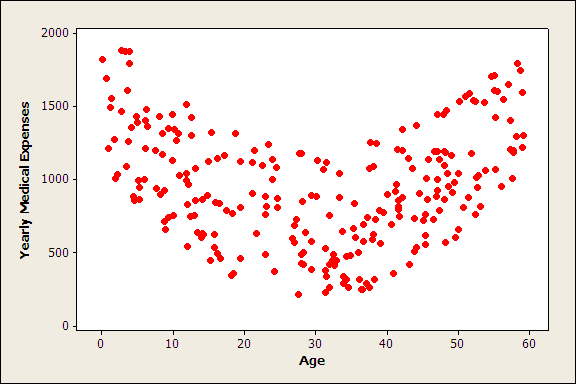
\includegraphics[width=0.5\textwidth]{smile.png}
			\end{center}
		\end{mcquestioninstruction}
		
		\question Which one of the following is a true statement about the data shown in the graph? \label{smile}
		\begin{mcanswerslist}
			\answer The correlation must be close to one because there is a strong relationship between age and medical expenses.
			\answer[correct] Using correlation on the data shown in the graph above is not appropriate because the relationship shown in the graph is not linear.
			\answer The direction of the association is positive.
			\answer There exist unusual observations in the plot above.
		\end{mcanswerslist}
		
		\begin{mcquestioninstruction}
			Data from the World Bank for 25 Western Hemisphere countries was used to examine the association between (average) female life expectancy (that is, the average lifespan of women in the country) and the average number of children women give birth to. Given below is the scatterplot for the data.
			\begin{center}
				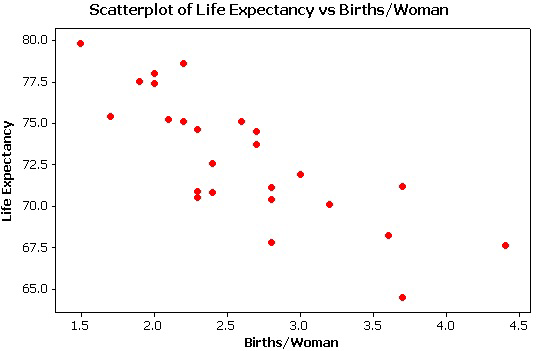
\includegraphics[width = 0.6 \textwidth]{life-birth.png}
			\end{center}
		\end{mcquestioninstruction}
		
		\question (6 points) The regression equation for this context is found to be \(\hat y = 84.5 - 4.4x\)
		where \(y\)
		is female life expectancy in years, and \(x\)
		is the average number of births per woman.   (a) Interpret the slope in context of the study and since this is observational data, (b) suggest a potential confounding variable and explain why it might be associated with both life expectancy and births/woman.
		\begin{mcanswerslist}[permutenone]
			\answer \rule{\textwidth}{0.5 pt}
			\rule{\textwidth}{0.5 pt}
			\answer \rule{\textwidth}{0.5 pt}
			\rule{\textwidth}{0.5 pt}
			\rule{\textwidth}{0.5 pt}
		\end{mcanswerslist}
		\begin{mcexplanation}
			The correct answers are
			\begin{enumerate}[label=(\alph*)]
				\item Expect to see a decrease of 4.4 years in female life expectancy when the average number of births per woman in a country increases by one child.
				\item Answers will vary.  Grade based on common sense and how detailed their explanation is.
			\end{enumerate}
		\end{mcexplanation}
		
		\begin{mcquestioninstruction}
			Annual measurements of the number of powerboat registrations (in thousands) and the number of manatees killed by powerboats in Florida were collected over the 14 years 1977–1990. A scatterplot of the data, least squares regression line, and correlation coefficient follow.  Use this situation to answer questions \ref{man-1}, \ref{man-2}, \ref{man-3}, and \ref{man-4}.
			\begin{center}
				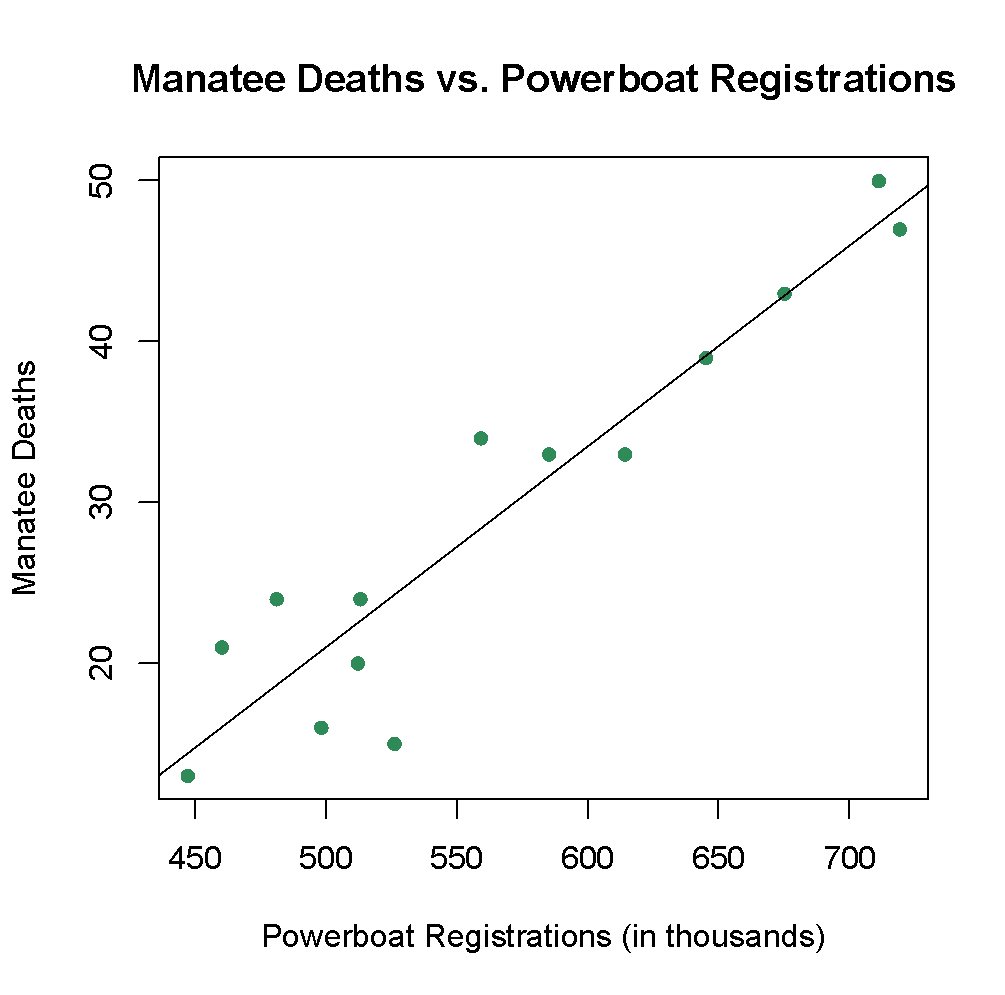
\includegraphics[width = 0.6\textwidth]{manatee.png} 				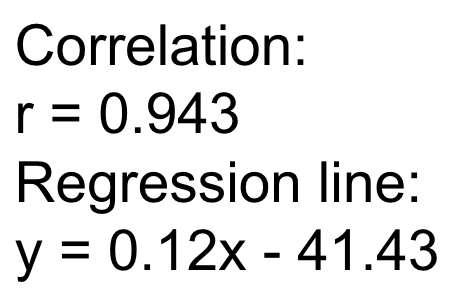
\includegraphics[width = 0.2\textwidth]{manatee-stats.png}
			\end{center}
		\end{mcquestioninstruction}
		
		\question What is the predicted number of manatee deaths for a year with 600,000 powerboat registrations? \label{man-1}
		\begin{mcanswerslist}
			\answer 0.12
			\answer[correct] 30.57
			\answer 4,143
			\answer 71,958.7
		\end{mcanswerslist}
		
		\question[follow] The y-intercept is not a valid prediction of manatee deaths. Why? \label{man-2}
		\begin{mcanswerslist}
			\answer It is an example of extrapolation. \label{man-ans-1}
			\answer[correct] Both \ref{man-ans-1} and \ref{man-ans-2}
			\answer We cannot observe a negative number of manatee deaths. \label{man-ans-2}
			\answer Another reason not stated here.
		\end{mcanswerslist}
		
		\question[follow] The year 1984 had 559,000 powerboat registrations and 34 manatee deaths. Did the least squares regression line underestimate, overestimate, or accurately estimate the number of manatee deaths for the year 1984? \label{man-3}
		\begin{mcanswerslist}
			\answer[correct] Underestimate
			\answer Overestimate
			\answer Accurately estimate
			\answer Cannot be determined
		\end{mcanswerslist}
		
		\question[follow] Which of the following is a correct interpretation of the coefficient of determination? \label{man-4}
		\begin{mcanswerslist}
			\answer About 94.3\% of the variation in manatee deaths can be explained by the number of powerboat registrations.
			\answer[correct] About 88.9\% of the variation in manatee deaths can be explained by the number of powerboat registrations.
			\answer An increase of 1,000 powerboat registrations is associated with a predicted increase of 0.943 manatee deaths.
			\answer An increase of 1,000 powerboat registrations is associated with a predicted increase of 0.889 manatee deaths.
		\end{mcanswerslist}
		
	\end{mcquestions}
\end{document}